\documentclass[a4paper]{article}
\usepackage[utf8]{inputenc}
\usepackage{amsmath}
\usepackage{amssymb}
\usepackage{mathtools}
\usepackage{amsfonts}
\usepackage{lastpage}
\usepackage{tikz}
\usepackage{float}
\usepackage{caption}
\usepackage{textcomp}
\usetikzlibrary{patterns}
\usepackage{pdfpages}
\usepackage{gauss}
\usepackage{fancyvrb}
\usepackage[table]{colortbl}
\usepackage{fancyhdr}
\usepackage{graphicx}
\usepackage[margin=2.5 cm]{geometry}

\definecolor{listinggray}{gray}{0.9}
\usepackage{listings}
\lstset{
	language=,
	literate=
		{æ}{{\ae}}1
		{ø}{{\o}}1
		{å}{{\aa}}1
		{Æ}{{\AE}}1
		{Ø}{{\O}}1
		{Å}{{\AA}}1,
	backgroundcolor=\color{listinggray},
	tabsize=3,
	rulecolor=,
	basicstyle=\scriptsize,
	upquote=true,
	aboveskip={0.2\baselineskip},
	columns=fixed,
	showstringspaces=false,
	extendedchars=true,
	breaklines=true,
	prebreak =\raisebox{0ex}[0ex][0ex]{\ensuremath{\hookleftarrow}},
	frame=single,
	showtabs=false,
	showspaces=false,
	showlines=true,
	showstringspaces=false,
	identifierstyle=\ttfamily,
	keywordstyle=\color[rgb]{0,0,1},
	commentstyle=\color[rgb]{0.133,0.545,0.133},
	stringstyle=\color[rgb]{0.627,0.126,0.941},
  moredelim=**[is][\color{blue}]{@}{@},
}

\lstdefinestyle{base}{
  emptylines=1,
  breaklines=true,
  basicstyle=\ttfamily\color{black},
}

\pagestyle{fancy}
\def\checkmark{\tikz\fill[scale=0.4](0,.35) -- (.25,0) -- (1,.7) -- (.25,.15) -- cycle;}
\newcommand*\circled[1]{\tikz[baseline=(char.base)]{
            \node[shape=circle,draw,inner sep=2pt] (char) {#1};}}
\newcommand*\squared[1]{%
  \tikz[baseline=(R.base)]\node[draw,rectangle,inner sep=0.5pt](R) {#1};\!}
\newcommand{\comment}[1]{%
  \text{\phantom{(#1)}} \tag{#1}}
\def\el{[\![}
\def\er{]\!]}
\def\dpip{|\!|}
\def\MeanN{\frac{1}{N}\sum^N_{n=1}}
\cfoot{Page \thepage\ of \pageref{LastPage}}
\DeclareGraphicsExtensions{.pdf,.png,.jpg}
\author{Nikolaj Dybdahl Rathcke (rfq695)}
\title{Machine Learning \\ Exam 2016}
\lhead{Machine Learning}
\rhead{Exam 2016}

\begin{document}
\maketitle

\section{The Traffic Sign Recognition Data}
\subsection{Question 1}
The method \texttt{makeFreqHistogram} implemented in python in the file \texttt{src/q1.py} produces a histogram showing the distribution of class frequencies given the number of bins and the classes of a dataset. Running \texttt{main.py}, will give us the histogram over the dataset \texttt{ML2015TrafficSignsTrain.csv} found in Figure \ref{fig1}.
\begin{figure}[H]
  \centering
  \captionsetup{justification=centering,margin=2cm}
  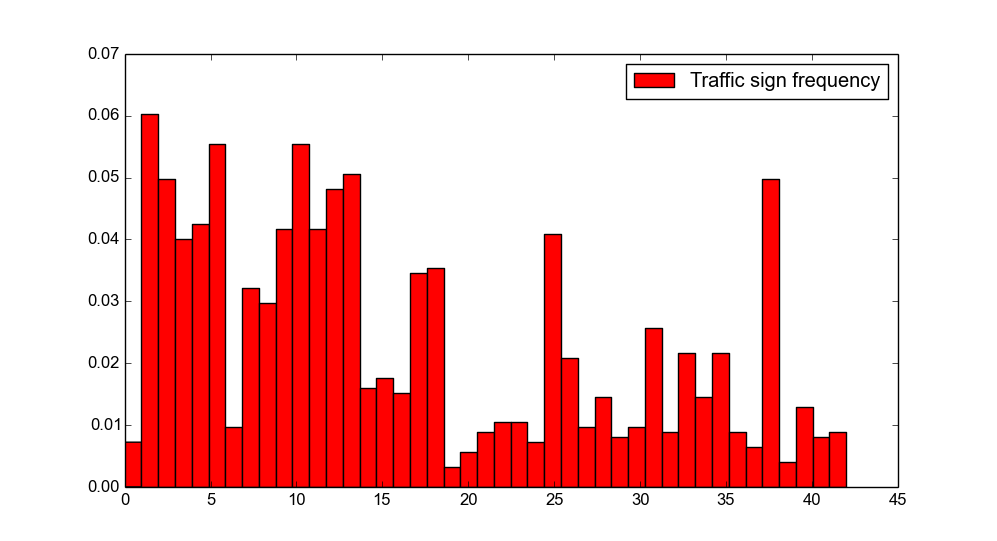
\includegraphics[scale=0.6]{histogram1}
  \caption{Histogram showing the distribution of class frequencies for the dataset \texttt{ML2015TrafficSignsTrain.csv}}
  \label{fig1}
\end{figure}
The histogram shows us that the number of observations for each class varies quite a bit.

\subsection{Question 2}
PCA has been implemented in python in \texttt{src/q1.py}. The function \texttt{pca} takes 2 arguments: The data and the classes corresponding to each entry in the data. Running \texttt{main.py} will produce the eigenspectrum and scatter plot for the dataset \texttt{ML2015TrafficSignsTrain.csv}. This produces Figure \ref{fig2} and \ref{fig3}. As a preprocessing step, the data has been normalized to zero mean and variance one.
\begin{figure}[H]
  \centering
  \captionsetup{justification=centering,margin=2cm}
  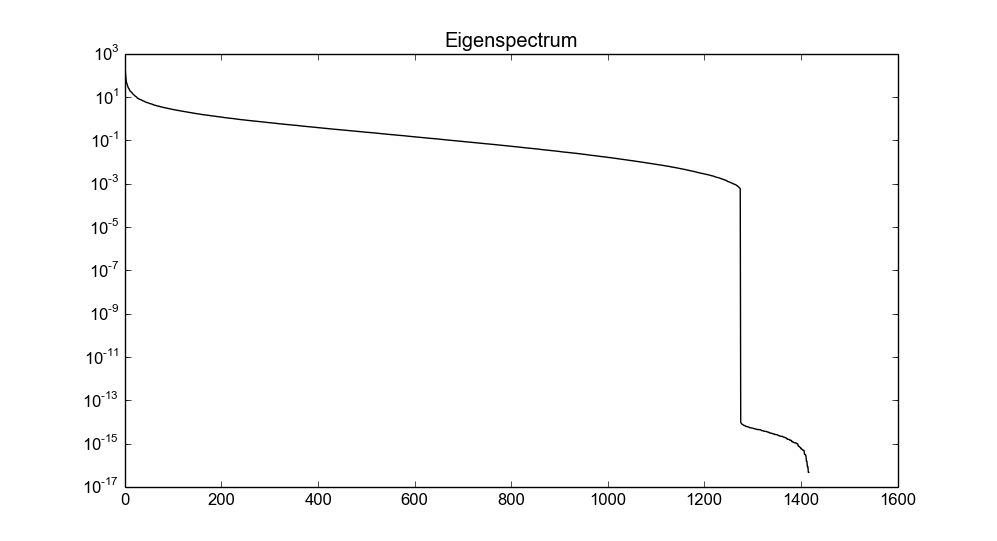
\includegraphics[scale=0.6]{eigenspectrum1}
  \caption{Eigenspectrum after performing PCA on the dataset \texttt{ML2015TrafficSignsTrain.csv}}
  \label{fig2}
\end{figure}
Besides the eigenspectrum, running the main file will also output how many principal components we need to explain $90\%$ of the variance to the terminal:
\begin{verbatim}
  Number of principal components to explain 90% of the variance:
  262
\end{verbatim}
So we need the 262 most influential principal components to explain $90\%$ of the variance.
\begin{figure}[H]
  \centering
  \captionsetup{justification=centering,margin=2cm}
  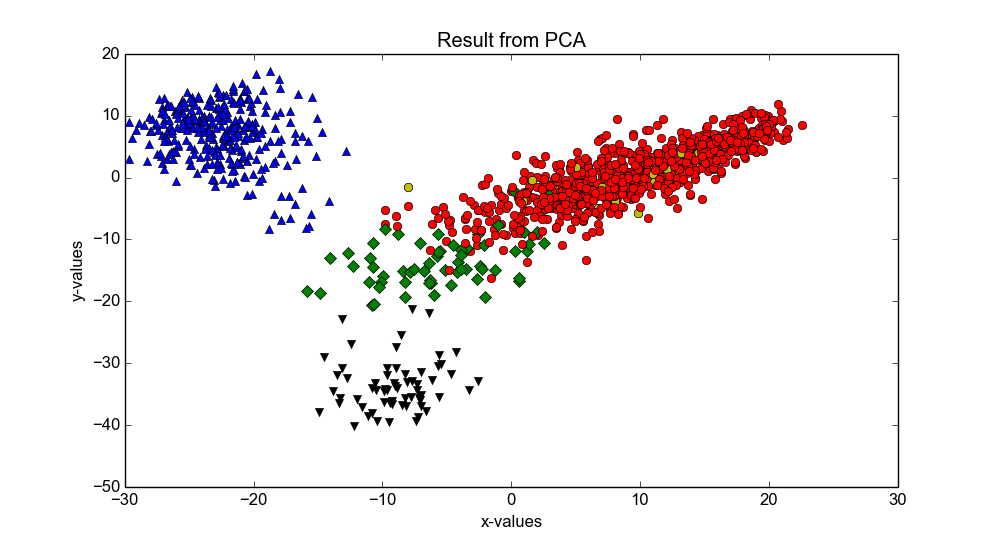
\includegraphics[scale=0.6]{scatter1}
  \caption{Scatter plot for the first two principal components where the colors (and shape) represent the shape of traffic signs. The scatter plot was generated from the dataset \texttt{ML2015TrafficSignsTrain.csv}}
  \label{fig3}
\end{figure}
The scatter plot shows us somewhat separable data. The yellow octagons are hard to separate from the red circles. This makes sense as a circle and an octagon have a close resemblance to each other. Some of the green square signs are mixed together with some of the circles, but all in all the data is divided quite well using only two principal components.

\subsection{Question 3}
K-means clustering has been implemented in python and is found in \texttt{src/q1.py}, which given a dataset, a $k$ representing the number of centroids and the classes, it will return the $k$ centroids after performing k-means. The function returns when the euclidean distance between the centroids in two consecutive iterations is less than the tolerance set to $0.0001$. Running \texttt{src/main.py} will produce Figure \ref{fig4} obtained from the dataset \texttt{ML2015TrafficSignsTrain.csv} and $k=4$. Again, the data has been normalized to zero mean and variance one.
\begin{figure}[H]
  \centering
  \captionsetup{justification=centering,margin=2cm}
  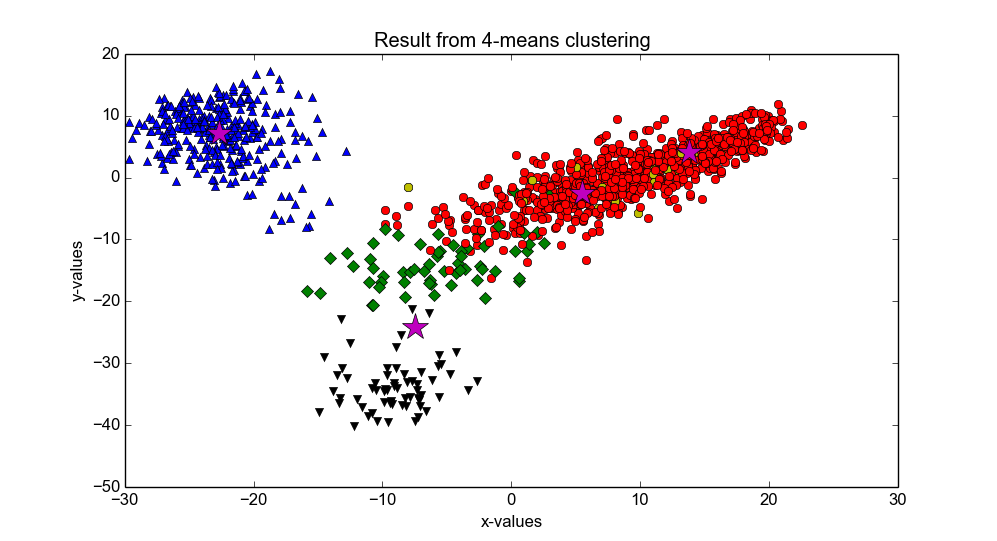
\includegraphics[scale=0.6]{scatter2}
  \caption{Scatter plot for the first two principal components with the $4$ centroids shown as purple stars. The plot is generated from the dataset \texttt{ML2015TrafficSignsTrain.csv}}
  \label{fig4}
\end{figure}
The centroids are represented by the purple stars. If we consider the reduction to two dimensions from PCA as an accurate measure for mutual distances, the centroids makes sense. Obviously, we would like to have a centroid for each shape (and one for circles and octagons), but there are two centroids for the circles/octagons and only one for both downward pointing triangles and diamonds. However, we have a lot of data points for circle shaped traffic signs, which means two of them might have a greater distance to each other than a diamond and a downward pointing triangle. This is also what the scatter plot reflects. Reducing the tolerance did not seem to affect the final centroids.

\section{Stars vs. Galaxies}
\subsection{Question 4}
The implementation is made in python and can be found in \texttt{src/q2.py} making use of the library \texttt{sklearn}. We first compute $\sigma_{Jaakkola}$ using the Jaakkola heuristic. We use $b=10$ for grid-search as this provided the best results, and we do $5$-fold cross validation. The training data has been normalized to zero mean variance one for the training data. The test data has been preprocessed, so that we use the mean and variance from the training data to normalize the test data. Running \texttt{main.py} will output the following to the terminal:
\begin{verbatim}
  Gamma value suggested by the Jaakkola Heuristic:
  0.461513538631

  Best parameters:
  {'kernel': 'rbf', 'C': 1000.0, 'gamma': 0.0046151353863122715}

  Success rate for training data:
  0.998666666667

  Success rate for test data:
  0.991333333333
\end{verbatim}
So our initial estimate $\gamma$ from Jaakkola's heuristic is roughly $0.46$. The optimal $C$ and $\gamma$ returned by grid-search is $1000$ and $0.0462$ respectively. With these parameters, the classification accuracy on the training data is $99.83\%$ and it is $99.13\%$ for the test data. This is quite a small error for both datasets.

\section{Normalization}
\subsection{Question 5}
Normalizing to zero mean and variance one before doing logistic regression is not needed, though it can help on the convergence for gradient descent. However, the regression should not change as we only scale the data. \\
Normalization to zero mean and variance one does nothing for random forests. The ranges do not really matter as a feature is never compared to another feature in terms of magnitude. So normalizing is unnecessary as it will not influence classification accuracy or choice of hyperparameters.

\section{Sparse Classifiers}
\subsection{Question 6}

\subsubsection{}
We are working with an infinite amount of hypotheses. Let $|S|=n$, let the expected loss of a hypothesis be $L(h)$ and the empirical error be $\hat{L}(h,S)$. Then by theorem $2.6$ in the lecture notes, we have that:
\begin{align}\label{ineq1}
  \mathbb{P}\left\{ \exists h \in \mathcal{H}:L(h)\geq \hat{L}(h, S)+\sqrt{\frac{8\ln(2((2n)^{d_{VC}}+1)/\delta)}{n}}\right\}\leq \delta
\end{align}
Now, we know that the VC-dimension for the hypothesis class of linear classifiers in $\mathbb{R}^d$ is $d+1$, so we get the following bound:
\begin{align*}
  \mathbb{P}\left\{ \exists h \in \mathcal{H}:L(h)\geq \hat{L}(h, S)+\sqrt{\frac{8\ln(2((2n)^{d+1}+1)/\delta)}{n}}\right\}\leq \delta
\end{align*}
Another way to read it is that we with probability at least $1-\delta$ for all $h\in\mathcal{H}$ have that:
\begin{align*}
  L(h)\leq \hat{L}(h,S)+\sqrt{\frac{8\ln(2((2n)^{d+1}+1)/\delta)}{n}}
\end{align*}
This means that no matter what $h$ is returned from the algorithm, we can with high probability have a guarantee on the expected performance.

\subsubsection{}
The coefficient $d$ should be relatively small compared to $n$ so the bound is not too loose. The smaller $d$ compared to $n$, the tighter the bound. \\
To avoid non-trivial information, we let $\delta=0.01$ to predict something with probability $99\%$. If we want a non-trivial information about the generalization error, we want the square root term to be less than $1$. If we ignore the constants (including $\delta$) in the square root term, we can derive the following relation between $d$ and $n$:
\begin{align*}
  \comment{Removing all constants} \mathcal{O}\left(\sqrt{\frac{8\ln(2((2n)^{d+1}+1)/\delta)}{n}}\right) &= \sqrt{\frac{\ln(n^d)}{n}}
\end{align*}
We want this to be less than $1$, so:
\begin{align*}
  &\sqrt{\frac{\ln(n^d)}{n}} < 1 \\
  \comment{Squaring both sides} &\Leftrightarrow \frac{\ln(n^d)}{n} < 1 \\
                                &\Leftrightarrow \ln(n^d) < n \\
  \comment{As we can assume $d,n > 0$} &\Leftrightarrow d\ln(n) < n \\
                                       &\Leftrightarrow d < \frac{n}{\ln n}
\end{align*}
So we want $d$ to be smaller than $\frac{n}{\ln n}$.

\subsubsection{}
Again we will use theorem 2.6 from the lecture notes with $d_{VC}=2$ as we are working in one dimension. However, there is a slight difference as we need to select a dimension as well. Thus, we have to use a union bound to provide an upper bound. Since we believe any dimension is as good as any other, we use $\delta_i$ to denote a distribution of our confidence budget $\delta$ among all subspaces $\mathcal{H}_{\{i\}}$, so $\delta_i=\frac{\delta}{d}$:
\begin{align*}
  &\mathbb{P}\left\{ \exists h \in \bigcup_{i=1}^d \mathcal{H}_{\{j\}} : L(h)\geq \hat{L}(h, S)+\sqrt{\frac{8\ln(2((2n)^{2}+1)/(\delta/d))}{n}}\right\} \\
   &\leq \sum_{i=1}^d \mathbb{P}\left\{ \exists h \in \mathcal{H}_{\{i\}} : L(h)\geq \hat{L}(h, S)+\sqrt{\frac{8\ln(2((2n)^{2}+1)/\delta_i)}{n}}\right\} \\
  \comment{Using inequality \ref{ineq1}} &\leq \sum_{i=1}^d \delta_i \\
  \comment{Substitute back for $\delta_i$} &=\sum_{i=1}^d \frac{\delta}{d} \\
                               &= \delta
\end{align*}
Last step is since we can replace the sum with $d$ and remove both $d$ terms in the fraction. This gives us a very nice and simple bound for learning with $\mathcal{H}_1^d$.

\subsubsection{}
Again we want the square root term to be less than $1$. We start by removing all the constants:
\begin{align*}
  \mathcal{O}\left(\sqrt{\frac{8\ln(2((2n)^{2}+1)/(\delta/d))}{n}}\right) = \sqrt{\frac{n^2d}{n}}
\end{align*}
And find the relation between $n$ and $d$:
\begin{align*}
  &\sqrt{\frac{\ln (n^2d)}{n}} < 1 \\
  &\Leftrightarrow \frac{\ln(n^2d)}{n} < 1 \\
  &\Leftrightarrow \ln(dn^2) < n \\
  &\Leftrightarrow dn^2 < e^n \\
  &\Leftrightarrow d < \frac{e^n}{n^2}
\end{align*}
Which means we want $d$ to be at least less than $e^n/n^2$.

\subsubsection{}
The proof follows the same lines as the proof from (4.1.3), but with a slightly different selection process. Like before, we want to distribute our confidence budget. Since we now pick $2$ dimension, we must distribute it to $\binom{d}{2}$ subspaces. Therefore we let $\delta_i=\frac{\delta}{\binom{d}{2}}$ and now we have $d_{VC}=3$. We also use a nested union bound now, so we get:
\begin{align*}
  &\mathbb{P}\left\{ \exists h \in \bigcup_{i=1}^d \bigcup_{j=i+1}^d \mathcal{H}_{\{i\}} : L(h)\geq \hat{L}(h, S)+\sqrt{\frac{8\ln(2((2n)^{3}+1)/(\delta/\binom{d}{2}))}{n}}\right\} \\
  &\leq \sum_{i=1}^d \sum_{j=i+1}^d \mathbb{P}\left\{ \exists h \in \mathcal{H}_{\{i\}} : L(h)\geq \hat{L}(h, S)+\sqrt{\frac{8\ln(2((2n)^{3}+1)/\delta_i)}{n}}\right\} \\
  \comment{Using inequality \ref{ineq1}} &\leq \sum_{i=1}^d\sum_{j=i+1}^d \delta_i \\
  \comment{Rewrite $\delta_i$} &=\sum_{i=1}^d \sum_{j=i+1}^d\frac{\delta}{\binom{d}{2}} \\
                               &= \delta
\end{align*}
Last step follows from simple combinatorics, as the double sum is the same as the triangular number to $d-1$ which is equal to $\binom{d}{2}$, and this gives us a bound for learning with $\mathcal{H}_2^d$.

\subsubsection{}
We want the square root term to be less than $1$. We start by removing the constants:
\begin{align*}
  \mathcal{O}\left(\sqrt{\frac{8\ln(2((2n)^{3}+1)/(\delta/\binom{d}{2}))}{n}}\right) = \sqrt{\frac{n^3d^2}{n}}
\end{align*}
The $d^2$ term comes from $\mathcal{O}\left(\binom{d}{2}\right)=d^2$. We can now find the relation between $n$ and $d$:
\begin{align*}
  &\sqrt{\frac{\ln (n^3d^2)}{n}} < 1 \\
  &\Leftrightarrow \frac{\ln(n^3d^2)}{n} < 1 \\
  &\Leftrightarrow \ln\left(n^3d^2\right) < n \\
  &\Leftrightarrow n^3d^2 < e^n \\
  &\Leftrightarrow d < \sqrt{\frac{e^n}{n^3}}
\end{align*}
Which means we want $d$ to be at least less than $\sqrt{\frac{e^n}{n^3}}$.

\subsubsection{}
The proof follows the same lines as the proof (4.1.5). This time, however, we do not know how many features we are looking at. To distribute our confidence budget, we let $\delta_i=\frac{\delta}{\binom{d}{\dpip h\dpip_0}}$. This means our VC-dimension is $\dpip h\dpip_0+1$. The union bound is a bit tricky. Since the bound essentially comes down to a counting problem, let $\bigcup_{\dpip h\dpip_0}$ denote the $\dpip h\dpip_0$ nested unions $\bigcup_{i=1}^d \bigcup_{j=i+1}^d \dots$ and so on. Similarly, let $\sum_{\dpip h\dpip_0}$ denote the nested sums. Then we can derive the following bound:
\begin{align*}
  &\mathbb{P}\left\{ \exists h \in \bigcup_{\dpip h\dpip_0} \mathcal{H}_{\{i\}} : L(h)\geq \hat{L}(h, S)+\sqrt{\frac{8\ln(2((2n)^{\dpip h\dpip_0+1}+1)/(\delta/\binom{d}{\dpip h\dpip_0}))}{n}}\right\} \\
  &\leq \sum_{\dpip h\dpip_0}\mathbb{P}\left\{ \exists h \in \mathcal{H}_{\{i\}} : L(h)\geq \hat{L}(h, S)+\sqrt{\frac{8\ln(2((2n)^{\dpip h\dpip_0+1}+1)/\delta_i)}{n}}\right\} \\
  \comment{Using inequality \ref{ineq1}} &\leq \sum_{\dpip h\dpip_0} \delta_i \\
  \comment{Rewrite $\delta_i$} &=\sum_{\dpip h\dpip_0}\frac{\delta}{\binom{d}{\dpip h\dpip_0}} \\
                               &= \delta
\end{align*}
The last step follows from combinatorics again as $\binom{d}{\dpip h\dpip_0}$ is the same as counting the nested sums, so they cancel each other out.

\subsubsection{}
Again, we start by taking O-notation of the square root term:
\begin{align*}
  \mathcal{O}(\sqrt{\frac{8\ln(2((2n)^{\dpip h\dpip_0+1}+1)/(\delta/\binom{d}{\dpip h\dpip_0}))}{n}}) = \sqrt{\frac{\ln(n^{\dpip h\dpip_0}\binom{d}{\dpip h\dpip_0})}{n}}
\end{align*}
We want it to be less than $1$, so we get:
\begin{align*}
  &\sqrt{\frac{\ln\left(n^{\dpip h\dpip_0}\binom{d}{\dpip h\dpip_0}\right)}{n}} < 1 \\
  &\Leftrightarrow \ln\left(n^{\dpip h\dpip_0}\binom{d}{\dpip h\dpip_0}\right) < n \\
  \comment{We use that $\binom{m}{k}\leq m^k$}  &\Leftrightarrow \ln\left(n^{\dpip h\dpip_0}d^{\dpip h\dpip_0}\right) < n \\
                                                &\Leftrightarrow (dn)^{\dpip h\dpip_0} < e^n \\
                                                &\Leftrightarrow \dpip h\dpip_0 \ln(dn) < e^n \\
  &\Leftrightarrow \dpip h\dpip_0 < \frac{e^n}{\ln(dn)}
\end{align*}
So $\dpip h\dpip_0$ has to be less than $e^n/\ln(dn)$.

\subsubsection{}
We start by taking O-notation of the square root term assuming $\dpip h\dpip_0=1$:
\begin{align*}
  \mathcal{O}(\sqrt{\frac{8\ln(2((2n)^{2}+1)/(\delta/\binom{d}{1}))}{n}}) = \sqrt{\frac{\ln(n^{2}\binom{d}{1})}{n}}
\end{align*}
We now find a relation between $n$ and $d$ to ensure it is smaller than $1$:
\begin{align*}
  &\sqrt{\frac{\ln\left(n^{2}\binom{d}{1}\right)}{n}} < 1 \\
  &\Leftrightarrow \ln\left(n^{2}\binom{d}{1}\right) < n \\
  \comment{Since $\binom{d}{1}=d$}  &\Leftrightarrow \ln\left(n^{2}d\right) < n \\
                                                &\Leftrightarrow n^2d < e^n \\
                                                &\Leftrightarrow d < \frac{e^n}{n^2}
\end{align*}
Which means $d$ must be smaller than the $e^n/n^2$ for the information on the generalization error to be non-trivial.

\subsubsection{}
Comparing the previous result with the result from (4.1.2), we see that $n/\ln(n)$ is a lot smaller than $e^n/n^2$. The bound on $\dpip h\dpip_0$ also enables $d$ to be larger than $n/\ln(n)$. This means that by working with sparse classifiers, we can work with more features ($d$) and still get a bound that is not trivial.

\subsubsection{}
Looking at the bound from (4.1.7), we see that increasing both $n$ and $d$ will drive number of features we can pick down. This is because the entire square root term will increase as well. Increasing $\delta$ however, will drive the number of features up as the square root term will be smaller. This makes sense, as $\delta$ is an indication of how certain we want to be. So if we want to be less certain that the bound is correct, we can make a tighter bound, which in turn allows us to pick more features out of $d$, while a looser bound will limit how many features we can pick.

\end{document}
